
% Copyright 2010, Tony R. Kuphaldt, released under the Creative Commons Attribution License (v 1.0)
% This means you may do almost anything with this work of mine, so long as you give me proper credit

%(BEGIN_FRONTMATTER)

\centerline{\bf Sequence of second-year Instrumentation courses}

\vskip 10pt

$$\includegraphics[width=15.5cm]{sequencex02.eps}$$  % 7-quarter schedule

\filbreak

The particular sequence of courses you take during the second year depends on when you complete all first-year courses and enter the second year.  Since students enter the second year of Instrumentation at four different times (beginnings of Summer, Fall, Winter, and Spring quarters), the particular course sequence for any student will likely be different from the course sequence of classmates.

Some second-year courses are only offered in particular quarters with those quarters not having to be in sequence, while others are offered three out of the four quarters and must be taken in sequence.  The following layout shows four typical course sequences for second-year Instrumentation students, depending on when they first enter the second year of the program:

$$\includegraphics[width=15.5cm]{sequencex01.eps}$$  % Sample schedules


\vfil

\underbar{file {\tt sequence}}
\eject
%(END_FRONTMATTER)


